% Options for packages loaded elsewhere
\PassOptionsToPackage{unicode}{hyperref}
\PassOptionsToPackage{hyphens}{url}
\PassOptionsToPackage{dvipsnames,svgnames,x11names}{xcolor}
%
\documentclass[
  a4paper,
]{article}

\usepackage{amsmath,amssymb}
\usepackage{iftex}
\ifPDFTeX
  \usepackage[T1]{fontenc}
  \usepackage[utf8]{inputenc}
  \usepackage{textcomp} % provide euro and other symbols
\else % if luatex or xetex
  \usepackage{unicode-math}
  \defaultfontfeatures{Scale=MatchLowercase}
  \defaultfontfeatures[\rmfamily]{Ligatures=TeX,Scale=1}
\fi
\usepackage{lmodern}
\ifPDFTeX\else  
    % xetex/luatex font selection
  \setmainfont[]{Arial}
\fi
% Use upquote if available, for straight quotes in verbatim environments
\IfFileExists{upquote.sty}{\usepackage{upquote}}{}
\IfFileExists{microtype.sty}{% use microtype if available
  \usepackage[]{microtype}
  \UseMicrotypeSet[protrusion]{basicmath} % disable protrusion for tt fonts
}{}
\makeatletter
\@ifundefined{KOMAClassName}{% if non-KOMA class
  \IfFileExists{parskip.sty}{%
    \usepackage{parskip}
  }{% else
    \setlength{\parindent}{0pt}
    \setlength{\parskip}{6pt plus 2pt minus 1pt}}
}{% if KOMA class
  \KOMAoptions{parskip=half}}
\makeatother
\usepackage{xcolor}
\usepackage[top=20mm,left=25mm,right=25mm]{geometry}
\setlength{\emergencystretch}{3em} % prevent overfull lines
\setcounter{secnumdepth}{-\maxdimen} % remove section numbering
% Make \paragraph and \subparagraph free-standing
\ifx\paragraph\undefined\else
  \let\oldparagraph\paragraph
  \renewcommand{\paragraph}[1]{\oldparagraph{#1}\mbox{}}
\fi
\ifx\subparagraph\undefined\else
  \let\oldsubparagraph\subparagraph
  \renewcommand{\subparagraph}[1]{\oldsubparagraph{#1}\mbox{}}
\fi


\providecommand{\tightlist}{%
  \setlength{\itemsep}{0pt}\setlength{\parskip}{0pt}}\usepackage{longtable,booktabs,array}
\usepackage{calc} % for calculating minipage widths
% Correct order of tables after \paragraph or \subparagraph
\usepackage{etoolbox}
\makeatletter
\patchcmd\longtable{\par}{\if@noskipsec\mbox{}\fi\par}{}{}
\makeatother
% Allow footnotes in longtable head/foot
\IfFileExists{footnotehyper.sty}{\usepackage{footnotehyper}}{\usepackage{footnote}}
\makesavenoteenv{longtable}
\usepackage{graphicx}
\makeatletter
\def\maxwidth{\ifdim\Gin@nat@width>\linewidth\linewidth\else\Gin@nat@width\fi}
\def\maxheight{\ifdim\Gin@nat@height>\textheight\textheight\else\Gin@nat@height\fi}
\makeatother
% Scale images if necessary, so that they will not overflow the page
% margins by default, and it is still possible to overwrite the defaults
% using explicit options in \includegraphics[width, height, ...]{}
\setkeys{Gin}{width=\maxwidth,height=\maxheight,keepaspectratio}
% Set default figure placement to htbp
\makeatletter
\def\fps@figure{htbp}
\makeatother
\newlength{\cslhangindent}
\setlength{\cslhangindent}{1.5em}
\newlength{\csllabelwidth}
\setlength{\csllabelwidth}{3em}
\newlength{\cslentryspacingunit} % times entry-spacing
\setlength{\cslentryspacingunit}{\parskip}
\newenvironment{CSLReferences}[2] % #1 hanging-ident, #2 entry spacing
 {% don't indent paragraphs
  \setlength{\parindent}{0pt}
  % turn on hanging indent if param 1 is 1
  \ifodd #1
  \let\oldpar\par
  \def\par{\hangindent=\cslhangindent\oldpar}
  \fi
  % set entry spacing
  \setlength{\parskip}{#2\cslentryspacingunit}
 }%
 {}
\usepackage{calc}
\newcommand{\CSLBlock}[1]{#1\hfill\break}
\newcommand{\CSLLeftMargin}[1]{\parbox[t]{\csllabelwidth}{#1}}
\newcommand{\CSLRightInline}[1]{\parbox[t]{\linewidth - \csllabelwidth}{#1}\break}
\newcommand{\CSLIndent}[1]{\hspace{\cslhangindent}#1}

\makeatletter
\makeatother
\makeatletter
\makeatother
\makeatletter
\@ifpackageloaded{caption}{}{\usepackage{caption}}
\AtBeginDocument{%
\ifdefined\contentsname
  \renewcommand*\contentsname{Table of contents}
\else
  \newcommand\contentsname{Table of contents}
\fi
\ifdefined\listfigurename
  \renewcommand*\listfigurename{List of Figures}
\else
  \newcommand\listfigurename{List of Figures}
\fi
\ifdefined\listtablename
  \renewcommand*\listtablename{List of Tables}
\else
  \newcommand\listtablename{List of Tables}
\fi
\ifdefined\figurename
  \renewcommand*\figurename{Figure}
\else
  \newcommand\figurename{Figure}
\fi
\ifdefined\tablename
  \renewcommand*\tablename{Table}
\else
  \newcommand\tablename{Table}
\fi
}
\@ifpackageloaded{float}{}{\usepackage{float}}
\floatstyle{ruled}
\@ifundefined{c@chapter}{\newfloat{codelisting}{h}{lop}}{\newfloat{codelisting}{h}{lop}[chapter]}
\floatname{codelisting}{Listing}
\newcommand*\listoflistings{\listof{codelisting}{List of Listings}}
\makeatother
\makeatletter
\@ifpackageloaded{caption}{}{\usepackage{caption}}
\@ifpackageloaded{subcaption}{}{\usepackage{subcaption}}
\makeatother
\makeatletter
\@ifpackageloaded{tcolorbox}{}{\usepackage[skins,breakable]{tcolorbox}}
\makeatother
\makeatletter
\@ifundefined{shadecolor}{\definecolor{shadecolor}{rgb}{.97, .97, .97}}
\makeatother
\makeatletter
\makeatother
\makeatletter
\makeatother
\ifLuaTeX
  \usepackage{selnolig}  % disable illegal ligatures
\fi
\IfFileExists{bookmark.sty}{\usepackage{bookmark}}{\usepackage{hyperref}}
\IfFileExists{xurl.sty}{\usepackage{xurl}}{} % add URL line breaks if available
\urlstyle{same} % disable monospaced font for URLs
\hypersetup{
  pdftitle={Comparison of Alzheimer's Disease research themes before and after lecanemab approval using text analysis of scientific literature},
  pdfauthor={Jess Scrimshire},
  colorlinks=true,
  linkcolor={blue},
  filecolor={Maroon},
  citecolor={Blue},
  urlcolor={Blue},
  pdfcreator={LaTeX via pandoc}}

\title{Comparison of Alzheimer's Disease research themes before and
after lecanemab approval using text analysis of scientific literature}
\author{Jess Scrimshire}
\date{2024-04-10}

\begin{document}
\maketitle
\ifdefined\Shaded\renewenvironment{Shaded}{\begin{tcolorbox}[borderline west={3pt}{0pt}{shadecolor}, interior hidden, enhanced, sharp corners, boxrule=0pt, frame hidden, breakable]}{\end{tcolorbox}}\fi

\renewcommand*\contentsname{Table of contents}
{
\hypersetup{linkcolor=}
\setcounter{tocdepth}{3}
\tableofcontents
}
\hypertarget{abstract}{%
\section{Abstract}\label{abstract}}

Every year thousands of scientific articles are published concerning the
chronic neurodegenerative disorder and leading cause of dementia,
Alzheimer's disease (AD). Currently there are no treatments that cure
AD, however the second anti-amyloid disease-modifying immunotherapy,
lecanemab, was granted accelerated approval by the FDA on 06-01-2023.
LDA topic modelling has previously been used to describe the AD research
landscape, however the effect of novel treatments has not been explored.
Using text mining and topic modelling, full abstract text between
01-01-2022 and 30-12-2023, and containing the MeSH term ``Alzheimer's
Disease'' from PubMed and preprint databases, were allocated to two
corpuses determined by the accelerated approval date for lecanemab.
Despite the frequency of literature increasing concerning terms relating
to lecanumab, topics mentioning neurodegeneration, study terminology,
and cellular and molecular pathologies have remained consistent
surrounding its approval. Increasing per-topic-per-word probabilities
for `tau' and `placebo' may suggest the research is shifting towards new
therapeutic targets and advances in later phase clinical trials, however
a longer follow up period will be necessary to validate these findings.

\hypertarget{introduction}{%
\section{Introduction}\label{introduction}}

\hypertarget{alzheimers-disease}{%
\subsection{Alzheimer's Disease}\label{alzheimers-disease}}

Alzheimer's disease (AD) is a chronic neurodegenerative disease
affecting over 55 million people worldwide, and is the most common cause
of dementia (1). The predominant symptoms of AD usually manifest after
the age of 65 and include cognitive impairment, physical and emotional
difficulties (2). The mechanisms determining the progression of AD are
not fully understood, but many agree on the amyloid or tau hypotheses,
originating from the presence of amyloid-beta (Aβ) plaques and
neurofibrillary tau tangles frequently found in the brains of patients
with AD (3,4). These abnormal proteins lead to disruptions in neuronal
signalling pathways and mediate cell death (5,6). Degeneration of the
hippocampus, which is a region vital for memory, and cortical atrophy
can leads to cognitive decline seen in AD (7,8).

AD diagnosis requires the presence of both amyloid and tau pathologies,
and signs of neuroinflammation, neuronal death and brain atrophy (9).
Biomarkers of neuroinflammation can be found in cerebrospinal fluid
(CSF) and blood plasma (10) or using brain imaging such as positron
emission tomography (PET) (11). Brain atrophy can be measured with
techniques such as magnetic resonance imaging (MRI) (12). Abnormal
protein deposits manifest in the brain before the onset of symptoms,
therefore early detection is required to prevent the spread of AD
pathologies and identify the right stage to administer treatments.

AD also has multiple risk factors suggesting age, epigenetic modifiers,
infectious agents, and diet all contribute to the development of AD
(13,14). An epidemiological comparison of people aged 65 years and older
from two different decades, suggested that the prevalence of AD is
decreasing due to an improvement in other lifestyle factors (15).
Observational studies are useful to identify other factors that are
important in the search to find treatments to target the key AD
pathologies.

\hypertarget{treatments-for-ad}{%
\subsection{Treatments for AD}\label{treatments-for-ad}}

There are currently no therapies or interventions that can cure AD, but
several approved treatments exist to manage cognitive impairment, to
alleviate symptoms, and enhance the overall quality of life for
patients. Acetylcholinesterase inhibitors (AchE) aim to increase the
levels of the neurotransmitter acetylcholine which are attenuated during
the pathologies of AD and associated with the loss of cholinergic
neurons (16). Whilst AchEs provide many benefits to treat the symptoms
of AD, they do not delay or stop the progression of the disease and the
effects may only last for 12-24 months (17). Mementine is a NMDA
receptor antagonist which inhibits glutamate mediated neurotoxicity
caused by neuronal cell death during AD progression (18). Memantine has
been approved for moderate severe to severe AD, however the drug has not
been shown to slow the progression of the disease or prove effective in
mild-to-moderate stages of the disease (19,20).

Two anti-amyloid human monoclonal immunotherapies, aducanumab and
lecanemab, have recently been granted approval by the United States Food
and Drug Administration (US FDA) which aim to reduce the Aβ plaques in
the AD brain (21,22). Aducanumab approval was rejected by the European
Medicines Agency (EMA) due to the conflicting phase III clinical trial
evidence and concerns over patient safety (23,24), whereas lecanumab is
currently under review by the EMA for approval (25). Aducanemab targets
the soluble Aβ oligomers and insoluble fibrils whereas lecanumab targets
the soluble Aβ protofibrils, but both led to the development of severe
adverse events including amyloid-related imaging abnormalities (ARIA)
(26,27). These results suggest further research is needed to understand
the full molecular causes of AD to help find safe yet effective
treatments.

Recent comprehensive reviews have identified a shift in research with
more Phase I studies being conducted and four more anti-amyloid
monoclonal antibody treatments having completing or currently undergoing
Phase III clinical trials (28,29). These trials are involving more
patients with early onset AD and mild cognitive impairment (MCI) to help
develop preventative therapies. Global estimates for people living with
preclinical AD or positive for AD pathology biomarkers were 69 and 315
million, respectively (30), therefore increasing research focus on these
patient populations is imperative to slow the progression of the
disease. These reviews have not been updated since the accelerated
approval of lecanemab, therefore we aim to identify whether there is a
transition in research topics with the emergence of these novel
disease-modifying treatments to target the underlying pathologies of AD
rather than treating the symptoms.

\hypertarget{text-mining-and-topic-modelling-in-ad-research}{%
\subsection{Text Mining and Topic Modelling in AD
Research}\label{text-mining-and-topic-modelling-in-ad-research}}

Thousands of articles are released every year concerning AD and the
Alzheimer's Association publishes an annual report to describe the
public health impact of AD for caregivers and society (2). Systematic
reviews and meta-analyses, however, are time consuming and labour
intensive, and pose a significant challenge to updating the current
understandings in the research literature (31). Topic modelling, an
unsupervised machine learning technique, can find patterns and
relationships within natural language data, and could provide an
automated and unbiased overview of research text. The most common topic
modelling method is Latent Dirichlet Allocation (LDA) which assumes, for
unstructured text data like research publication, that each document is
made up of a number of topics and that each topic is made up of a
collection of words (32). Each LDA topic is represented as a probability
of words within a topic and a probability of topics within each
document, which each follow a Dirichlet distribution.

\emph{In silico} topic modelling has been used for various applications
relating to AD, including identifying novel biomarkers (33), and drug
repurposing (34). LDA has also been used to describe trends in the
research landscape, however this has only been achieved until 01-01-2022
(35,36). Guan \emph{et al} (36) identified fourteen clusters from
abstract text from 95,876 papers published between 2007 and 2016 with
the entry term `Alzheimer's Disease'. Topics included the burden of AD
such as `cost' and `health' as well as protein terminology such as `APP'
which related to the amyloid-precursor protein which is cleaved into
amyloid-beta via the amyloidogenic pathway (37). Martinelli (35)
performed a nine-topic LDA model and identified five mechanistic themes,
one topic relating to AD diagnosis and three concerning treatments.
Whilst both descriptive analyses using LDA topic modelling have
identified key topics in AD research, further research was suggested to
validate their findings.

To the best of our knowledge, no studies have described the AD research
landscape since this period and explored whether the emergence of newly
approved immunotherapy treatments have affected research themes. We
therefore aimed to comprehensively characterise AD research through the
period that the AD drug, lecanemab, underwent accelerated approval for
early AD on 06-01-2023 . We hypothesised that new treatments targeting
the pathophysiological changes in patients with AD represent a major
paradigm shift in AD research. We proposed that LDA topic models could
summarise the latest research and help identify distinct thematic
changes in the literature. Furthermore, this method could help
understand the complexities of AD and be translated to other
neurodegenerative diseases to study the impact of emerging novel
treatments.

\newpage{}

\hypertarget{methods}{%
\section{Methods}\label{methods}}

A full summary of the methodology is provided in
Figure~\ref{fig-full-summary}. All data analysis and visualisations were
done in R version 4.3.2 using \emph{tidyverse} packages (38) unless
otherwise stated.

\begin{figure}

{\centering 

\begin{figure}[H]

{\centering 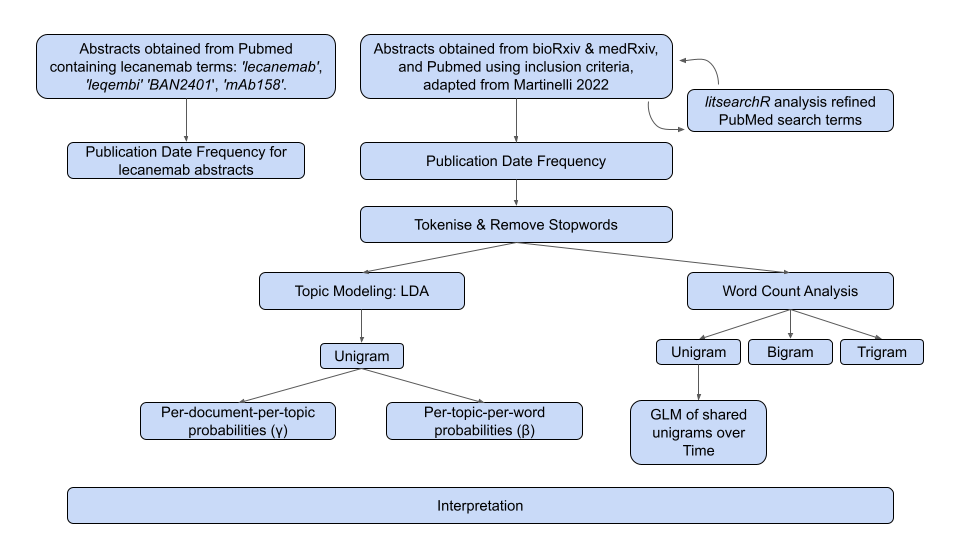
\includegraphics[width=3.2in,height=\textheight]{data/methodsummary.png}

}

\end{figure}

}

\caption{\label{fig-full-summary}\textbf{Summary of methods.} Abstracts
gathered from PubMed then updated with \emph{litsearchr} results, or
from preprint databases were read into R. Metadata analysis was
performed then text was tidied and tokenised, then allocated to two
corpuses relative to the accelerated approval date of lecanemab. LDA
topic modelling and n-gram analysis were performed then results were
interpreted.}

\end{figure}

\hypertarget{data-acquisition}{%
\subsection{Data Acquisition}\label{data-acquisition}}

Due to accessing constraints, abstracts represent the only document
content for this study. Titles, full abstract text, and publication date
were obtained from the National Center for Biotechnology Information
(NCBI) datasbase, PubMed, using the inclusion criteria described in
Table~\ref{tbl-inclusion-criteria}, and accessed through \emph{Rismed}
(39) on 18-02-2024. Results from PubMed were combined with publications
from the preprint data sources, bioRxiv and medXriv, using
\emph{medrxiv} (40). Entries were assigned Medical Subject Headings
(MeSH) which identified health-related terms within each document,
therefore classifying articles according to their subject nature. An
additional dataset was generated for abstracts containing the associated
terminology for the AD drug lecanemab: `\emph{lecanemab}',
`\emph{leqembi}' `\emph{BAN2401}', and `\emph{mAb158}'.

\newpage{}

\hypertarget{tbl-inclusion-criteria}{}
\begin{longtable}[]{@{}
  >{\raggedright\arraybackslash}p{(\columnwidth - 2\tabcolsep) * \real{0.3718}}
  >{\raggedright\arraybackslash}p{(\columnwidth - 2\tabcolsep) * \real{0.6282}}@{}}
\caption{\label{tbl-inclusion-criteria}\textbf{Inclusion criteria used
to query and identify all relevant terms concerning AD in the PubMed
database.} Adapted from Martinelli (35).}\tabularnewline
\toprule\noalign{}
\begin{minipage}[b]{\linewidth}\raggedright
Criteria
\end{minipage} & \begin{minipage}[b]{\linewidth}\raggedright
Filter Applied
\end{minipage} \\
\midrule\noalign{}
\endfirsthead
\toprule\noalign{}
\begin{minipage}[b]{\linewidth}\raggedright
Criteria
\end{minipage} & \begin{minipage}[b]{\linewidth}\raggedright
Filter Applied
\end{minipage} \\
\midrule\noalign{}
\endhead
\bottomrule\noalign{}
\endlastfoot
MeSH Term & `Alzheimer's Disease' \\
Title and/or Abstract Text & `Alzheimer's Disease'

`AD' \\
Article Type & ``Books''

``Case Reports''

``Clinical Study''

``Clinical Trial''

``Controlled Clinical Trial''

``Meta-analysis''

``Randomised Controlled Trial''

``Review''

``Systematic Review'' \\
Publication Date & 1st January 2022 to 1st January 2024 inclusive \\
Language & English \\
\end{longtable}

\hypertarget{litsearchr}{%
\subsubsection{\texorpdfstring{\emph{litsearchR}}{litsearchR}}\label{litsearchr}}

To reassure us that the PubMed search query encapsulated all literature,
we used \emph{litsearchr} to automate identifying search terms and
reduce bias in the initial keyword selection by using co-occurrence
networks (41). Citations from the PubMed results, using the previous
search criteria in Table~\ref{tbl-inclusion-criteria}, were read into R.
The combined unique keyword and titles, as not all articles have
keywords, for each result were collected. To ensure only the most
relevant terms were searched, stop words were removed as these contained
very frequent terms that provided no significant information, such as
`the', `and' or `a'. The minimum frequency of words for keywords and
title was then set to n = 50 and n = 75, respectively. A
document-frequency matrix of each search term in each article was
created and computed into a co-occurrence network using
\emph{create\_network} (42). The potential search terms were ranked
using \emph{strength} (43) and the change point method calculated the
optimal cutoff positions where the strength of the next strongest term
was greater than the previous one.

\hypertarget{data-preprocessing}{%
\subsection{Data Preprocessing}\label{data-preprocessing}}

Abstracts and their metadata were categorised into two corpuses:
`Pre-Lecanemab Accelerated Approval' and `Post-Lecanemab Accelerated
Approval', based on their publication date relative to the date of
lecanemab's accelerated early approval, 06-01-2023 (22). Full abstract
text was tokenised into one-, two- and three-word tokens using
\emph{tidytext} (44) (Figure~\ref{fig-preprocess-1}). Stop words,
combined with the words frequent to the unigram analysis,
``\emph{alzheimer's}'' and ``\emph{ad}'', were then removed
(Figure~\ref{fig-preprocess-2}). To prevent the different spellings of
the same phrase from being counted multiple times, similar bigrams and
trigrams were mapped to the same variable. For example, `\emph{amyloid
β}, `\emph{beta amyloid}', and `\emph{amyloid aβ}' were all mapped to
`\emph{amyloid beta}', and `\emph{mild cognitive impairments}' and
`\emph{cognitive impairment mci}' were mapped to `\emph{mild cognitive
impairment}'. Additionally, for bigrams originating from trigrams,
mapping to the first two terms was used or mapping to an acronym, for
example `\emph{central nervous}' and `\emph{system cns'} were mapped
to'\emph{cns}'.

\begin{figure}

{\centering 

\begin{figure}[H]

{\centering 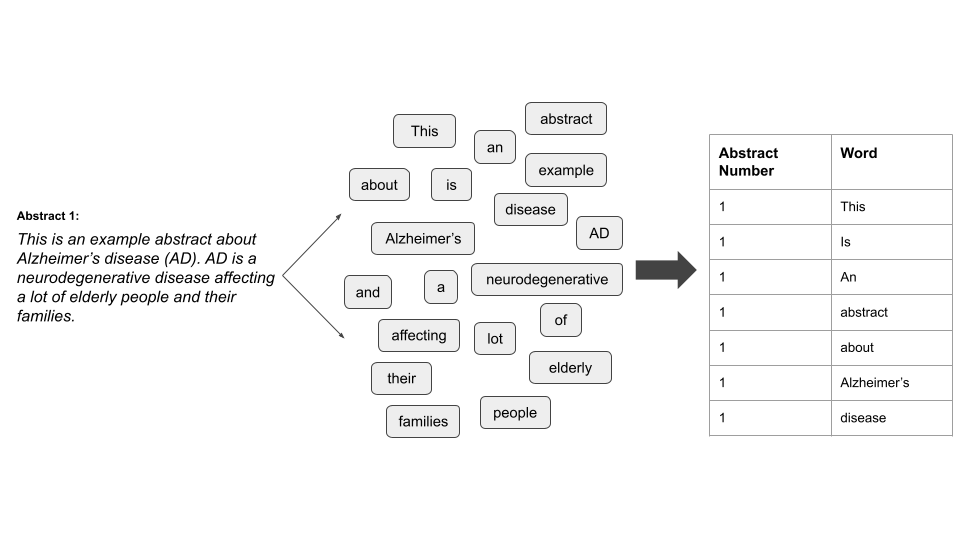
\includegraphics[width=3.2in,height=\textheight]{data/preprocess1.png}

}

\caption{Unigram Tokenisation.}

\end{figure}

\begin{figure}[H]

{\centering 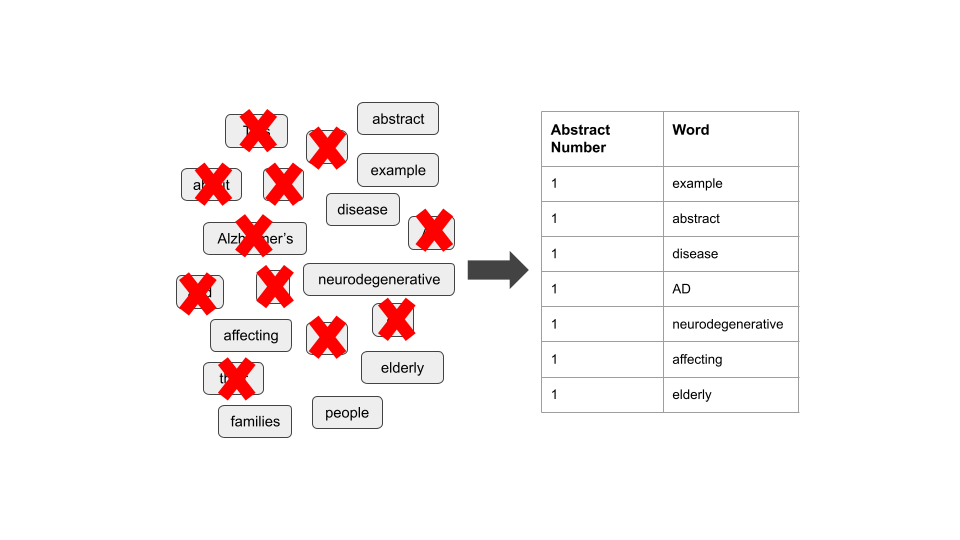
\includegraphics[width=3.2in,height=\textheight]{data/preprocess2.png}

}

\caption{Removal of Stop Words.}

\end{figure}

}

\caption{\label{fig-preprocess}\textbf{Abstract preprocessing into
unigrams.} Schematic of an abstract being (A) tokenised into single-word
tokens followed by (B) removal of stop words and personalised words
frequent to the unigram analysis, `\emph{alzheimers}', and `\emph{AD}'.
Tokenisation and data cleaning of bigrams and trigrams followed the same
methods, not shown.}

\end{figure}

\hypertarget{data-analysis}{%
\subsection{Data Analysis}\label{data-analysis}}

\hypertarget{frequency-analysis}{%
\subsubsection{Frequency Analysis}\label{frequency-analysis}}

The frequency of all eligible abstracts published per month as well as
the frequency of publications containing the associated terminology for
the AD drug lecanemab were visualised.

After tokenisation, the top 15 most frequent unigrams were determined
for each dataset. The top 15 most frequent bigrams and trigrams were
also determined due to many unigrams being associated with pairs or
triplets of words. For example, ``\emph{mild cognitive impairment}''
relates to a neurological condition, whereas the words ``\emph{mild}'',
``\emph{cognitive}'' and ``\emph{impairment}'' have ambiguous
connotations individually. A generalised linear model (GLM) was used to
determine whether there was a significant change in word usage per
months for the most frequent unigrams shared by both corpuses.

\hypertarget{topic-modelling}{%
\subsubsection{Topic Modelling}\label{topic-modelling}}

A document term matrix (dtm) was constructed for each dataset,
indicating each word's term frequency (tf), which is a measure of how
often a word appears in each abstract. To determine if a statistical
model could distinguish between the text corpuses surrounding the
accelerated approval date of lecanemab, a two-topic Latent Dirich
Allocation (LDA) model (32) was applied to the dtm using
\emph{topicmodels} (45). The per-document-per-topic probabilities (γ)
was extracted to show the proportion of words generated in each topic
and how often these words appear in either corpuses.

Two ten-topic LDA models were also created, one for each text corpuses,
to determine the most frequent topics. In each model the abstracts were
considered mixtures of topics and each topic was considered a mixture of
words. The per-topic-per-word probabilities (β) were extracted and the
top 10 terms most common words found in each topic were visualised.
Topic titles were manually created and validated by a neuroscience
expert.

\hypertarget{results-and-discussion}{%
\section{Results and Discussion}\label{results-and-discussion}}

The final dataset contained 6744 abstracts that were published between
01-01-2022 and 30-12-2023 (Figure~\ref{fig-results-summary}).

\begin{figure}

{\centering 

\begin{figure}[H]

{\centering 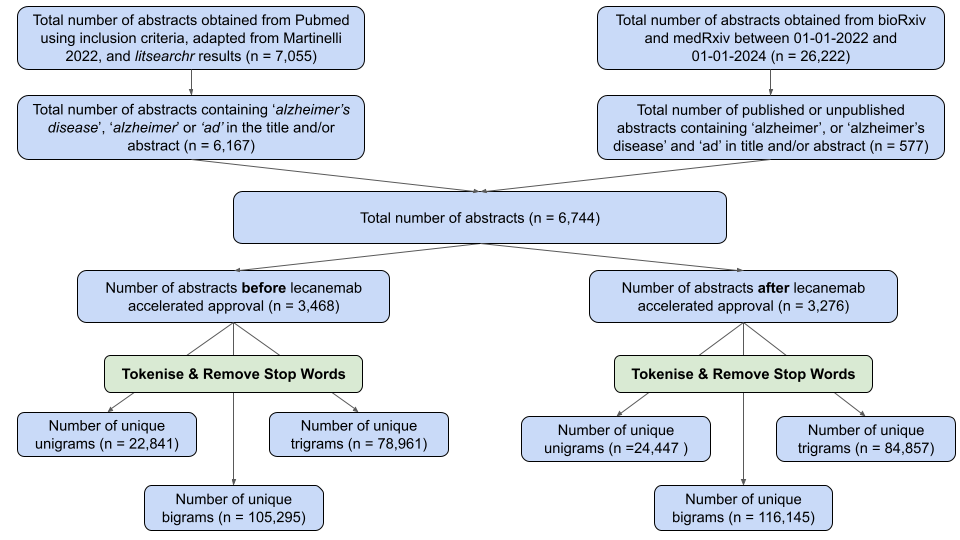
\includegraphics[width=3.2in,height=\textheight]{data/resultsummary.png}

}

\end{figure}

}

\caption{\label{fig-results-summary}\textbf{Summary of abstracts and
n-grams used for analysis}. Counts for abstracts obtained from PubMed
and preprint databases were allocated to two corpuses based on their
publication date relative to the accelerated approval date of lecanemab,
06-01-2023. Frequencies for unique n-grams after tokenisation and
stop-word removal were calculated.}

\end{figure}

\hypertarget{search-query-refinement-identified-the-term-alzheimer}{%
\subsection{Search Query Refinement Identified the Term
`alzheimer'}\label{search-query-refinement-identified-the-term-alzheimer}}

Our initial search query was refined using \emph{litsearchr} (41) to
determine the most important terms to the articles ranked by their
strength (Figure~\ref{fig-ad-search-terms}). We disregarded
`\emph{alzheimer's disease}' as this MeSH term was included in the
original search query, but we updated the PubMed search query with
`\emph{alzheimer}' (Table~\ref{tbl-inclusion-criteria}). We omitted the
unigram `\emph{disease}' as this term was too broad and may have
encapsulated articles concerning other irrelevant neurodegenerative
diseases into our query. We inclued English articles only, which are
estimated to be about 75\% of the scientific literature (46).

Due to our search strategy, a lot of papers containing the MeSH term
`Alzheimer's disease' may have been mentioned as a collective with other
neurodegenerative diseases. MeSH terms are added manually to articles in
PubMed, therefore there could be an interpretive bias when authors add
these to their publications. We tried to avoid this by filtering the
titles and abstracts of PubMed articles to also contain the term
`\emph{alzheimer's disease}', `\emph{ad}' or `\emph{alzheimer}'.
Similarly when MeSH terms were not available for the bioRxiv and medRxv
databases, we used a similar search strategy to filter titles and
abstract text to contain the term `\emph{alzheimer's disease}' or
`\emph{alzheimer}', or `\emph{ad}' and `\emph{alzheimer's disease}'.
This filtering may have biased our dataset as abstracts not containing
these search terms were omitted despite the full article text
potentially concerning AD, however abstract text has previously been
used to identify themese in AD literature (36). We would, however,
suggest that further studies use full article text to help validate our
findings.

\begin{figure}

{\centering 

\begin{figure}[H]

{\centering 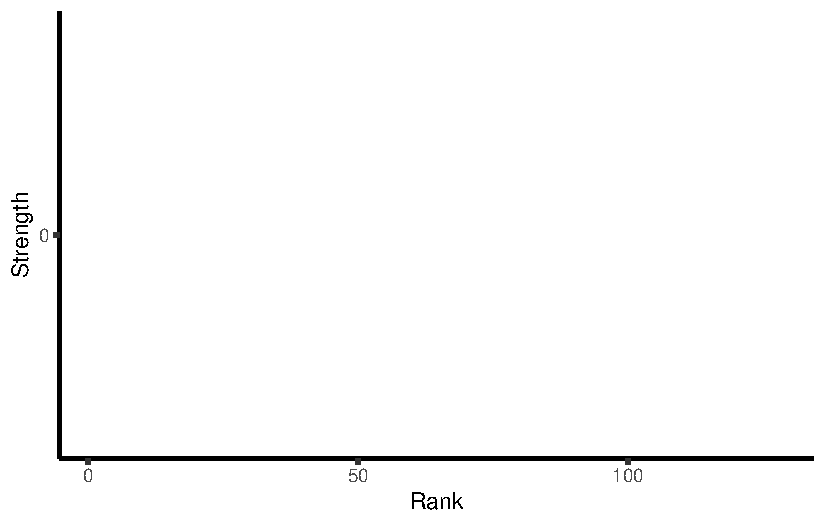
\includegraphics{report_pdf_files/figure-pdf/fig-ad-search-terms-1.pdf}

}

\end{figure}

}

\caption{\label{fig-ad-search-terms}\textbf{Search query refinement
using \emph{litsearchr} identified `\emph{alzheimer}'.} A matrix of each
word in each article was created and the potential search terms were
ranked with \emph{create\_network} and \emph{strength} (42) from the
\emph{igraph} package (43). The dashed lines mark the optimal cutoff
positions where the strength of the next strongest term was greater than
the previous one. The top keywords and words from the titles of AD
papers, with minimum frequencies of n = 50 and n = 75, respectively,
were ranked by their importance to article content then the top terms
were considered to refine the original search query, adapted from
Martinelli (35).}

\end{figure}

\hypertarget{increased-lecanemab-publication-frequency-did-not-impact-ad-research-topics}{%
\subsection{Increased lecanemab publication frequency did not impact AD
research
topics}\label{increased-lecanemab-publication-frequency-did-not-impact-ad-research-topics}}

Lecanemab received accelerated and traditional approval in 2023 (22,47),
however we did not find any variability in the overall frequency of
literature published containing the MeSH term `\emph{Alzheimer's
Disease}', with 3,468 abstracts published before and 3,276 abstracts
published after the accelerated approval of lecanemab
(Figure~\ref{fig-results-summary}, Figure~\ref{fig-publication-date-1}).
Despite the frequency of publications containing the terms associated
with the AD drug lecanemab exponentially increasing in 2023
(Figure~\ref{fig-publication-date-2}), there was no significant
difference between the per-document-per-topic probabilities (γ) for the
two-topic LDA models (Figure~\ref{fig-gamma-lda}). This suggests that
the increase in abstracts concerning lecanemab did not separate the
literature into two distinct topics based on differing themes.

\begin{figure}

\begin{minipage}[t]{0.50\linewidth}

{\centering 

\begin{figure}[H]

{\centering 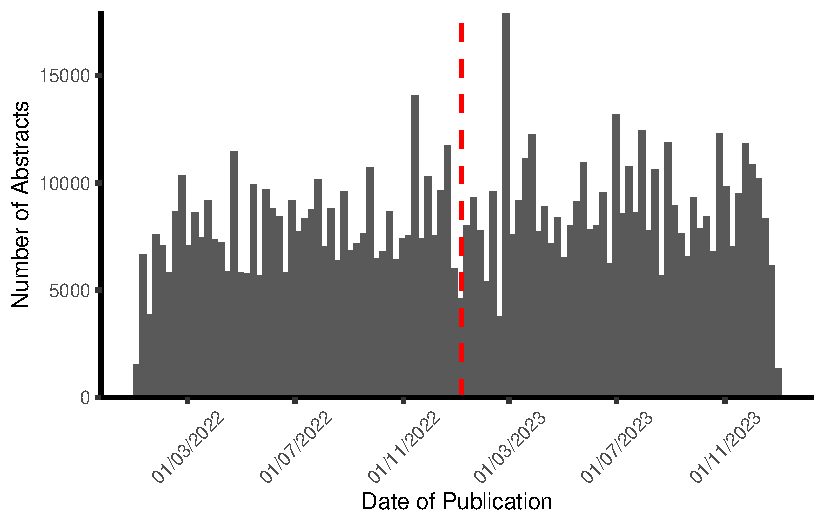
\includegraphics{report_pdf_files/figure-pdf/fig-publication-date-1.pdf}

}

\caption{All Abstracts}

\end{figure}

\begin{figure}[H]

{\centering 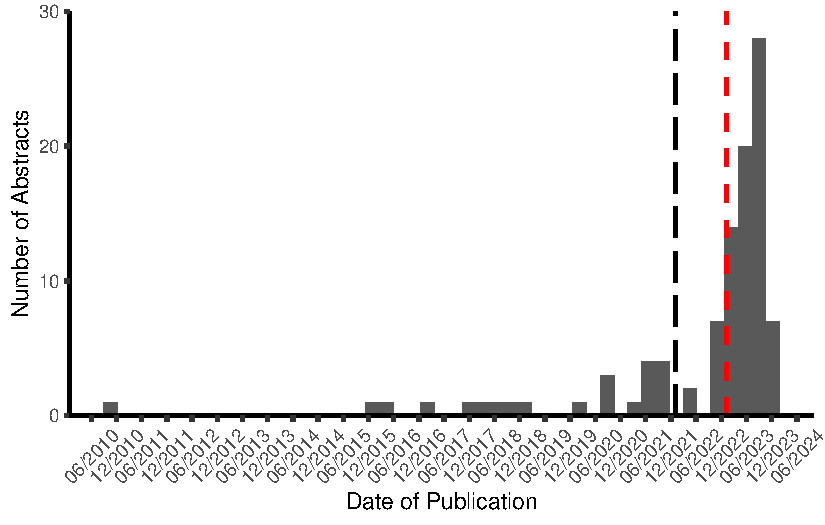
\includegraphics{report_pdf_files/figure-pdf/fig-publication-date-2.pdf}

}

\caption{Lecanemab Abstracts}

\end{figure}

}

\end{minipage}%

\caption{\label{fig-publication-date}\textbf{Increase in lecanemab
publications does not change AD publication frequency.} Distribution of
articles published over time containing (A) the MeSH term `Alzheimer's
Disease' in the title and/or abstract (n = 6744) or (B) terms associated
with the AD drug lecanemab: `\emph{lecanemab}', `\emph{leqembi}',
`\emph{BAN2401}', and `\emph{mAb158}' (n = 202). Black long-dashed line
represented the start of our observation period. Red dashed-line
represents date of lecanemab accelerated approval, 06-01-2023.}

\end{figure}

\newpage{}

One reason for there not being any statistical significance between the
per-document-per-topic probabilities could be due to the two-year time
period being too short to account for a change in the research
landscape, as previous studies have used a five-year or ten-year time
period to characterise topics in AD literature (36). Whilst no studies
have compared LDA topics in two time periods, changes in AD research may
take multiple years to manifest. Further research should explore a
larger time period after the accelerated approval of lecanemab to
conclude whether a change in the research literature can be found using
topic models.

\begin{figure}

{\centering 

\begin{figure}[H]

{\centering 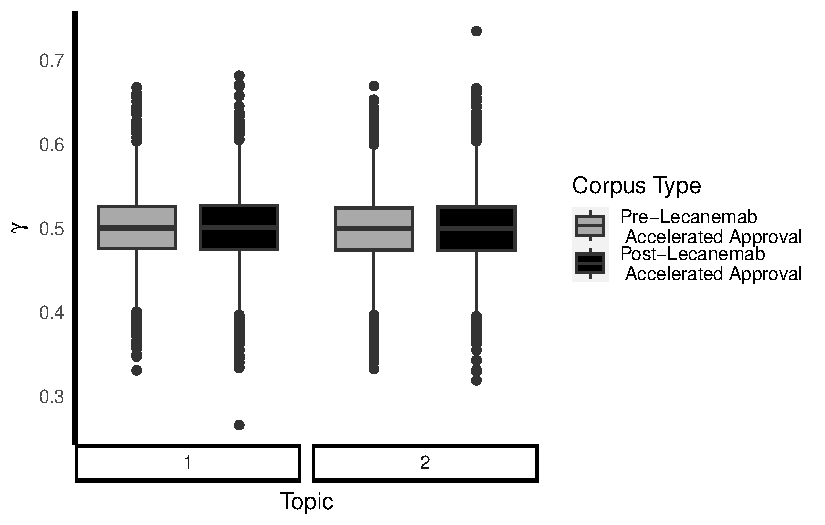
\includegraphics{report_pdf_files/figure-pdf/fig-gamma-lda-1.pdf}

}

\end{figure}

}

\caption{\label{fig-gamma-lda}\textbf{Two topic LDA model does not
distinguish change in literature around accelerated approval date of
Lecanemab}. A document term matrix (dtm) was constructed for the unigram
dataset and a two topic LDA model was applied to the dtm using
\emph{topicmodels} (45). Boxplots show first and third quartiles, median
and outlier per-document-per-topic probabilities, γ. Corpus type was
determined based on accelerated approval date for lecanemab, 06-01-2023.
n = 6744.}

\end{figure}

\hypertarget{neurodegeneration-and-cognitive-impairment-are-associated-with-ad-research}{%
\subsection{``Neurodegeneration'' and ``cognitive impairment'' are
associated with AD
research}\label{neurodegeneration-and-cognitive-impairment-are-associated-with-ad-research}}

Despite the full abstract dataset not significantly splitting into two
distinct topics, we suggested this was because the language was very
similar between the two corpses. We therefore explored the most common
n-grams frequencies. Fourteen of the fifteen most frequent unigrams were
shared between the two corpuses (Figure~\ref{fig-tokenisation-1}),
however there were no significant differences between the unigram
frequencies between the two time periods
(Figure~\ref{fig-tokenisation-4}). Similarly, fourteen of the fifteen
most frequent bigrams and trigrams were shared between the two corpuses
(Figure~\ref{fig-tokenisation-2}, Figure~\ref{fig-tokenisation-3}). This
suggested that the word usage has remained consistent and indicated that
the introduction of a novel anti-amyloid therapy may not have changed
the research landscape. We used LDA topic modelling to see whether the
terms may be distributed differently in different topics in each corpus.
Identifying ten topics per corpus and the top ten keywords per topic, we
found topics concerning neurodegeneration, study terminology or related
to AD pathology were shared by the two corpuses
(Figure~\ref{fig-topic-model-unigrams}).

\begin{figure}

{\centering 

\begin{figure}[H]

{\centering 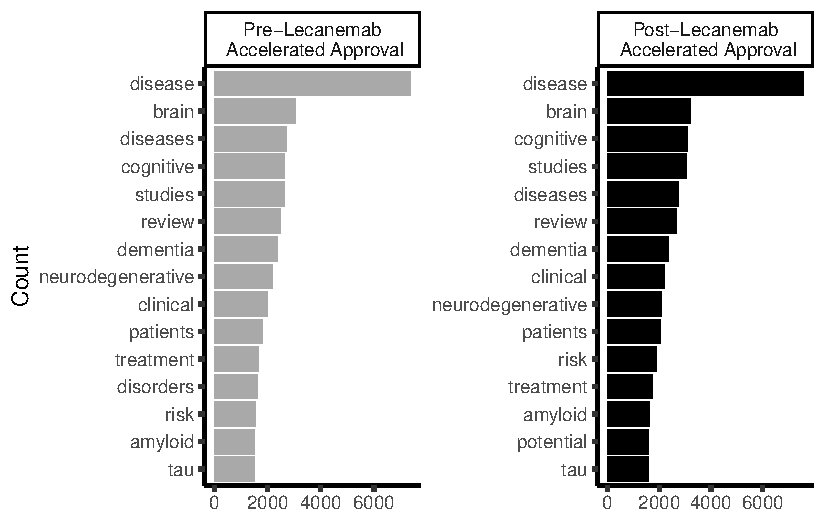
\includegraphics{report_pdf_files/figure-pdf/fig-tokenisation-1.pdf}

}

\caption{Unigram}

\end{figure}

\begin{figure}[H]

{\centering 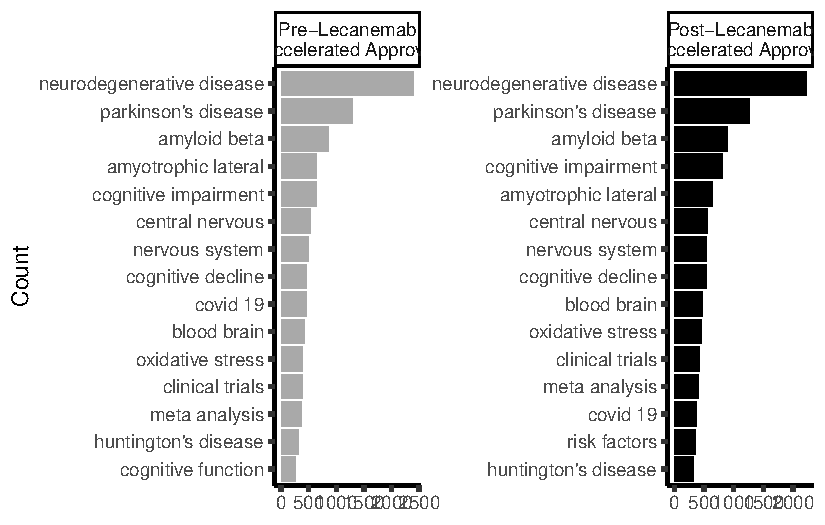
\includegraphics{report_pdf_files/figure-pdf/fig-tokenisation-2.pdf}

}

\caption{Bigram}

\end{figure}

\begin{figure}[H]

{\centering 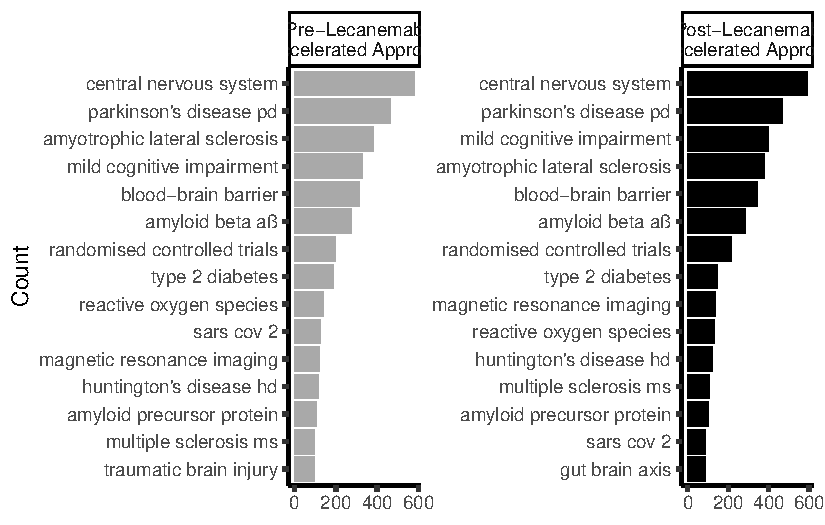
\includegraphics{report_pdf_files/figure-pdf/fig-tokenisation-3.pdf}

}

\caption{Trigram}

\end{figure}

\begin{figure}[H]

{\centering 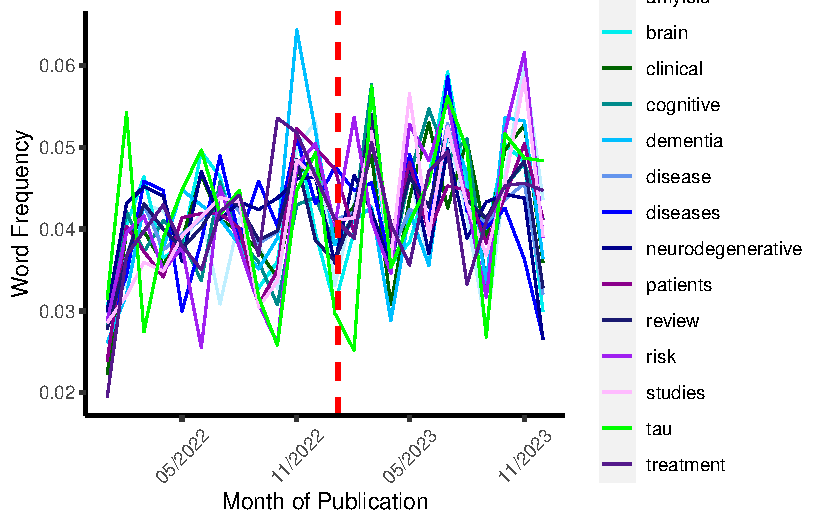
\includegraphics{report_pdf_files/figure-pdf/fig-tokenisation-4.pdf}

}

\caption{Most common words}

\end{figure}

}

\caption{\label{fig-tokenisation}\textbf{Literature use is similar
around the time of lecanemab approval.} Corpus type was determined based
on accelerated approval date for lecanemab, 06-01-2023 then tokenised
and removal of stop words. The 15 most frequent (A) unigrams, (B)
bigrams and (C) trigrams along with (D) the distribution by month of the
top 14 shared most frequent unigrams for both corpuses (n = 6744).
Dashed-line represents the accelerated approval date of lecanemab,
06-01-2023.}

\end{figure}

`\emph{Disease}' was the most frequent unigram in both corpuses
(Figure~\ref{fig-tokenisation-1}) and was included with
`\emph{neurodegenerative disease}', `\emph{Parkinson's disease
{[}pd{]}}' and `\emph{Huntington's disease {[}hd{]}}', which were among
the most frequent bigrams and trigrams
(Figure~\ref{fig-tokenisation-2}, Figure~\ref{fig-tokenisation-3}).
Similar topics in both corpuses were classified by terms co-occurring
with `\emph{cognitive}', included `\emph{memory}', `\emph{sleep}',
`\emph{impairment}' and `\emph{brain}' or `\emph{learning}' and
\emph{`dementia\emph{'. While '}neurodegenerative'} was common to three
topics per corpus, '\emph{parkinson's'} was the only specific disease
observed co-occurring in a topic in the earlier corpus, and none in the
later corpus. Parkinson's disease (PD) is another common
neurodegenerative disease caused by neuronal loss and affects
coordination and motor skills. The drug development pipeline for PD
contains fewer trials than for AD, however 36 new studies for PD were
initiated in the year prior to lecanemab which could attribute to its
occurrence in this topic corpus (28,48).

\hypertarget{genetic-risk-of-apoe-in-ad}{%
\subsection{Genetic risk of APOE in
AD}\label{genetic-risk-of-apoe-in-ad}}

Genetic risk as well as other AD-related risk factors were common to LDA
topics in both corpuses. The terms `\emph{genes', 'genetic}', and
\emph{'risk}' were shared by both models, however `\emph{covid}' and
`\emph{19}' were unique to the earlier corpus
(Figure~\ref{fig-topic-model-unigrams}). A genetic link has been
hypothesised between having COVID-19 and developing AD (49,50), and we
observed `\emph{covid 19}' and `\emph{sars cov 2}' were also among the
most frequent bigram and trigrams
(Figure~\ref{fig-tokenisation-2}, Figure~\ref{fig-tokenisation-3}). The
frequency of COVID-19-related n-grams was greater in the earlier corpus,
however we cannot conclude whether this is a consequence of the large
volume of COVID-19-related research published during the pandemic, or a
causal links to AD.

The rare dominantly inherited AD (DIAD) is caused by mutations in the
amyloid precursor protein (APP) gene and genes for the presenilin 1 and
presenilin 2 proteins (51). We only found `\emph{amyloid precursor
protein}' referenced in the n-gram analysis, however the gene
`\emph{APOE}' occurred in LDA topics in both corpuses
(Figure~\ref{fig-tokenisation-3}, Figure~\ref{fig-topic-model-unigrams}).
Apolipoprotein E (APOE) is the most significant risk gene for late-onset
AD and associated with age-related cognitive decline (52,53).

\begin{figure}

{\centering 

\begin{figure}[H]

{\centering 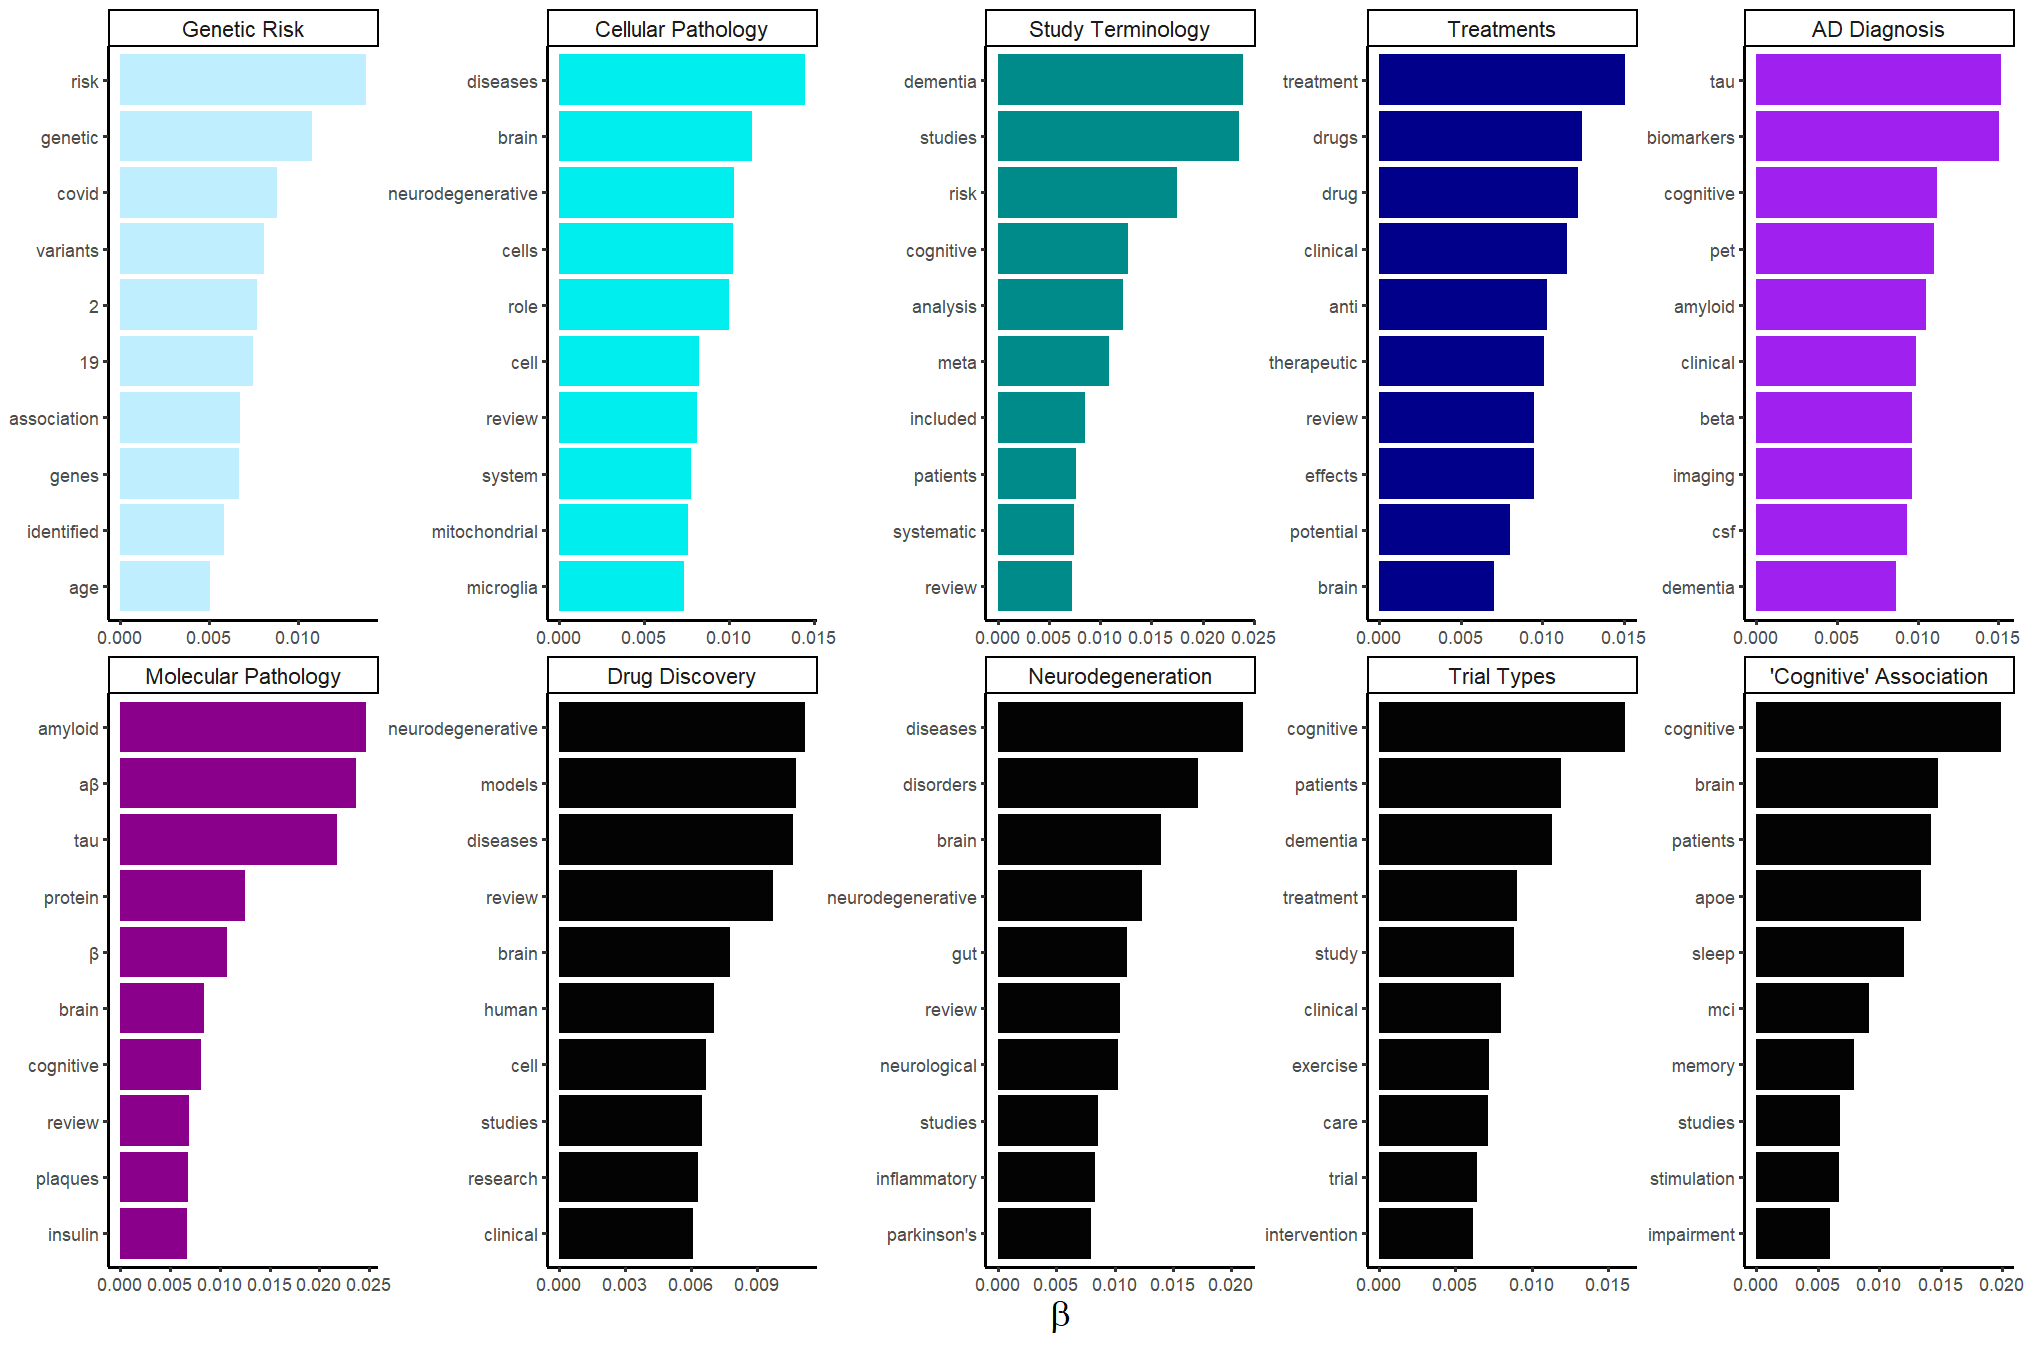
\includegraphics[width=6.75in,height=\textheight]{plots/pre-leca-lda-updated-blue2.png}

}

\caption{Pre-Lecenamab Accelerated Approval: Top 10 unigrams in each LDA
topic}

\end{figure}

\begin{figure}[H]

{\centering 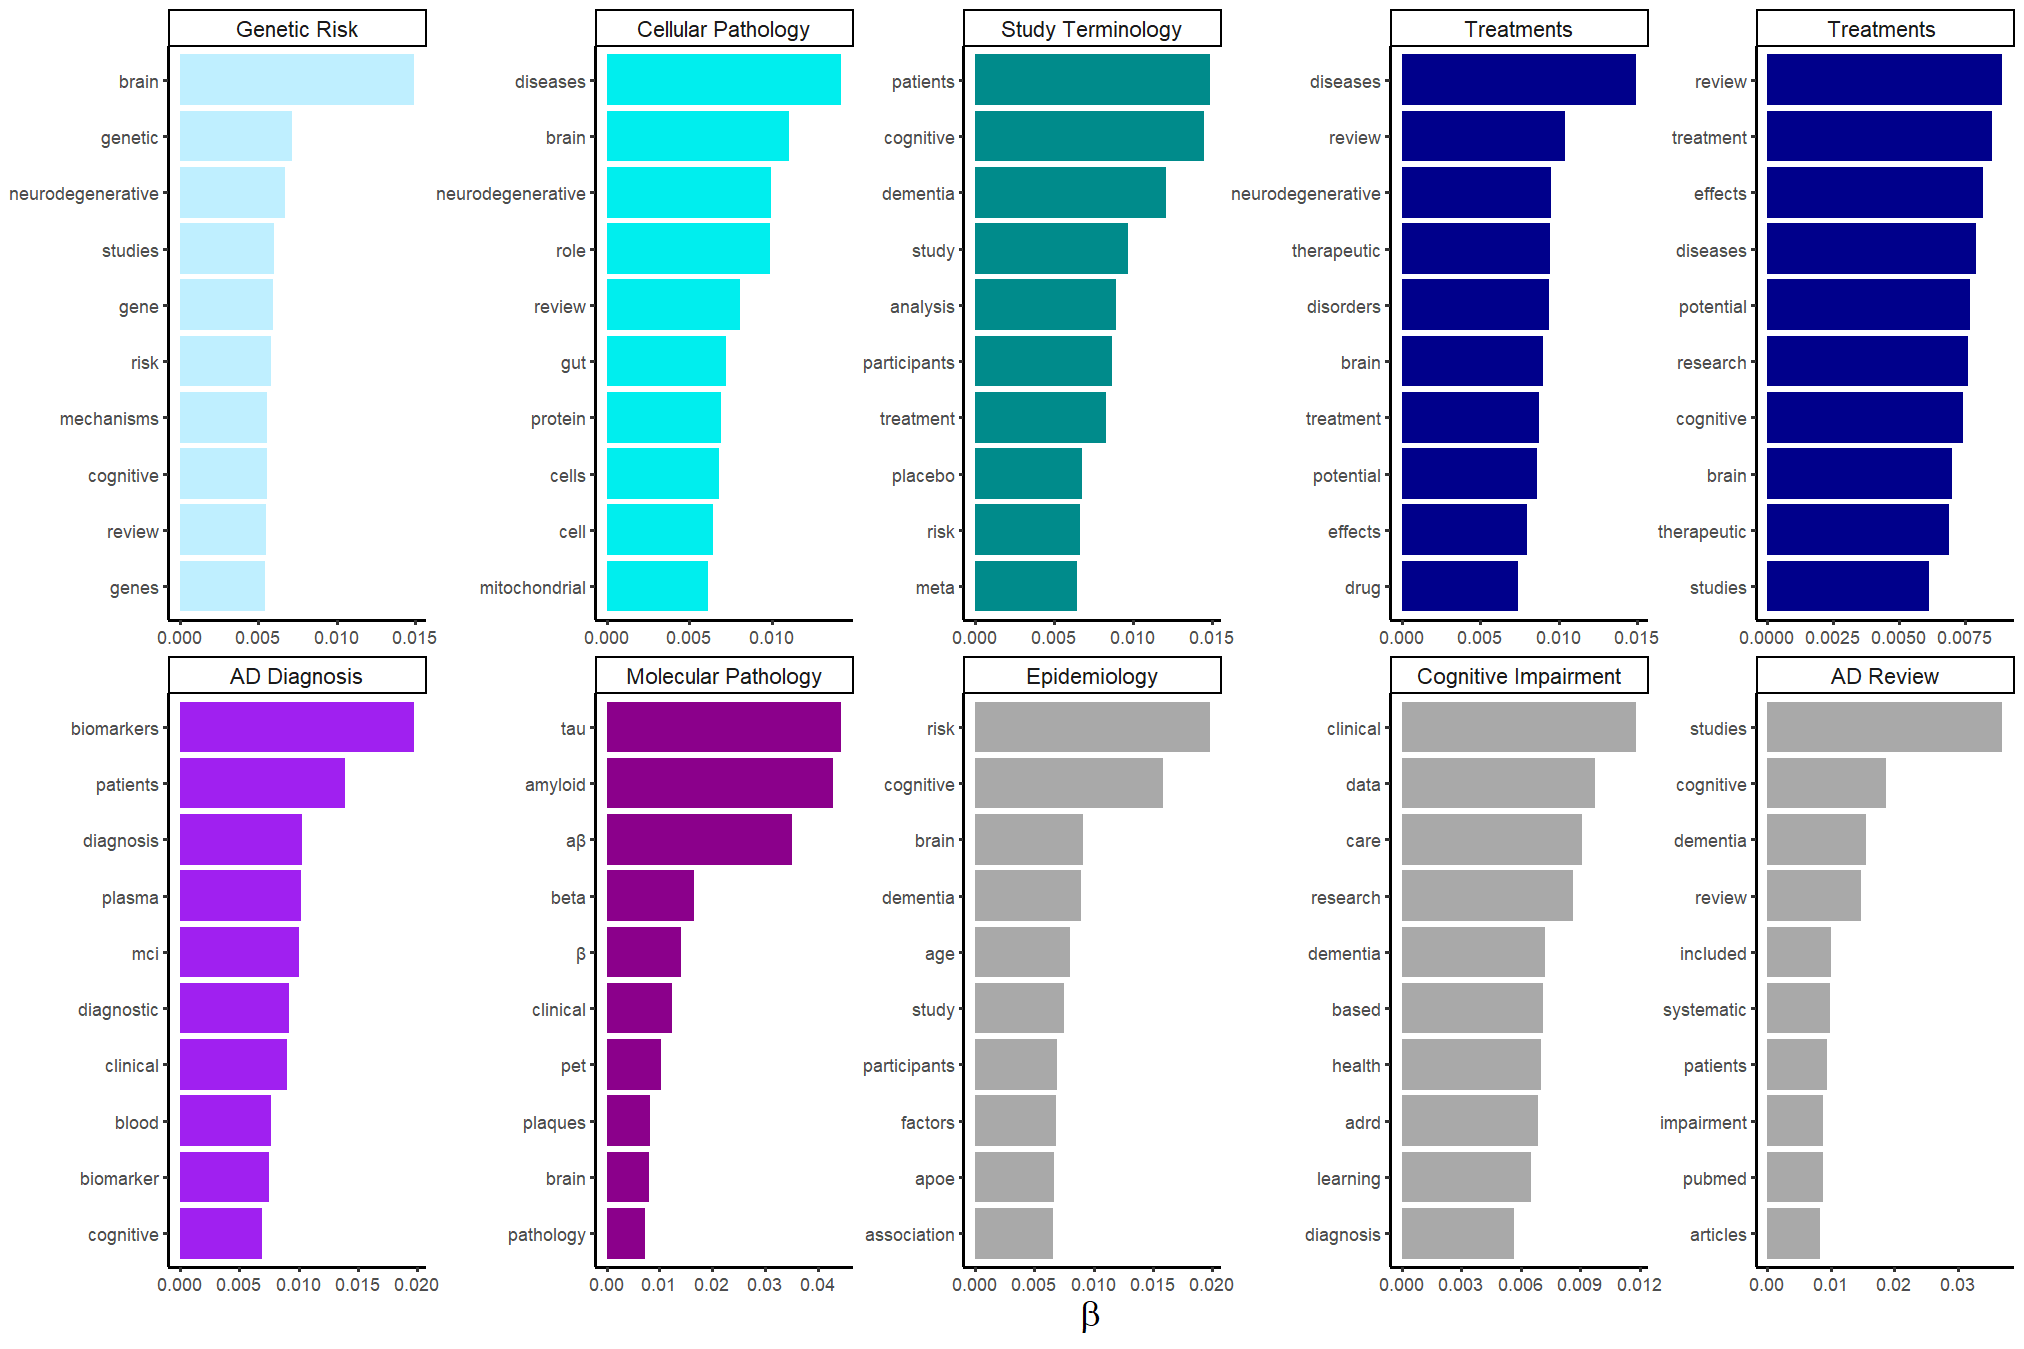
\includegraphics[width=6.75in,height=\textheight]{plots/post-leca-lda-updated-blue2.png}

}

\caption{Post-Lecanemab Accelerated Approval: Top 10 unigrams in each
LDA topic}

\end{figure}

}

\caption{\label{fig-topic-model-unigrams}\textbf{LDA topic models
concern neurodegeneration, study terminology and pathology surrounding
lecanemab accelarated approval.} Outputs from the ten-topic LDA model
for abstracts published (A) before and (B) after the accelerated
approval date of lecenamab, 2023-01-06. The top 10 unigrams per topic
are ordered by their per-topic-per-word probability, β. Topic titles
were manually created and validated with a neuroscience expert. Topic
colours matched when the same topic was identified in (A) then (B).}

\end{figure}

\hypertarget{tau-research-may-be-increasing-after-lecanemab-accelerated-approval}{%
\subsection{Tau research may be increasing after lecanemab accelerated
approval}\label{tau-research-may-be-increasing-after-lecanemab-accelerated-approval}}

Topics containing study terminology were common to both corpuses,
however the unigram `\emph{placebo}' was unique to the later corpus
(Figure~\ref{fig-topic-model-unigrams}). The frequency of the trigram
`\emph{randomised controlled trials}' was greater in the later corpus
(Figure~\ref{fig-tokenisation-3}), despite fewer abstracts being in this
dataset (Figure~\ref{fig-results-summary}). This could suggest an
increase in the number of randomised clinical trials (RCT) after
lecanemab received accelerated approval . Placebos are used when there
is no known or FDA-approved therapy that can be tolerated by patients,
therefore as AD does not have a standard of care treatment to cure the
disease, a placebo may be used in RCTs. This is consistent with the
trends observed in Huang \emph{et al} (29), which suggested an increase
in Phase III clinical trials for anti-amyloid therapies in 2023 which
encompassed the traditional approval date of lecanemab by the FDA in
July 2023 from the CLARITY AD clinical trial (47).

Multiple topics in the earlier corpus referenced study terminology and
trial types, either relating to pre-clinical drug discovery in
`\emph{cells}' and `\emph{models}' or clinical studies such as
`\emph{trials}', `\emph{human}'. There were two topics relating to
treatments after the accelerated approval of lecanemab and only one
before, however language use was similar with the mention of
`\emph{drug}', \emph{`potential\emph{', and }'effects\emph{' being
observed (Figure~\ref{fig-topic-model-unigrams}). Whilst topics in the
AD literature have previously mentioned clinical outcomes (35), mention
of randomised clinical trials and placebo-controlled trials have not
emerged using LDA topic models. There was an increase in the beta-value
for the terms '}tau'}, '\emph{amyloid',} and \emph{`aβ'} in the topic
concerning molecular pathology after the accelerated approval of
lecanemab. Clinical trials including disease-modifying therapies
targeting tau have increased with 14 active trials at the beginning of
2023 (28), therefore research may be shifting to the other pathological
hypotheses of AD to identify treatments.

\hypertarget{immunological-and-metabolic-research-in-ad}{%
\subsection{Immunological and metabolic research in
AD}\label{immunological-and-metabolic-research-in-ad}}

As the cause of AD is not full understood, topics concerning the
molecular pathology, specifically referencing `\emph{amyloid-beta}' and
`\emph{tau}', were found and highlighted the importance of these
hypotheses. Topics concerning cellular pathology and mentioning
`\emph{migroglia}' and `\emph{mitochondrial}' may referred to the
increased neuroinflammation relating to the recruitment of immune cells
in AD (Figure~\ref{fig-topic-model-unigrams}). We also found mentions of
`\emph{oxidative stress}' and '\emph{reactive oxygen species'} in both
corpuses in the n-gram analysis (Figure~\ref{fig-tokenisation-2}).
Mitochondria produce reactive oxygen species and initiate neuronal cell
death in AD (54). Microglia are important as part of the innate immune
response to remove Aβ, however tau pathologies may induce an
inflammatory state in microglia causing the phagocytosis of synapses and
secretion of neurotoxic cytokines (55,56).

The term `\emph{insulin}' was only found in the earlier corpus
(Figure~\ref{fig-topic-model-unigrams}), however '\emph{type 2
diabetes'} was one of the most common trigrams for both corpuses
(Figure~\ref{fig-tokenisation-3}). AD has been referred to as type 3
diabetes due to the rapid growth of literature concerning brain insulin
resistance and experimental evidence has shown insulin sensitiser
treatments may help attenuate learning deficits (57--60). Many
epidemiological studies have suggested T2DM may be increasing the risk
of AD, leading to the lower brain insulin levels resulting in decreased
clearance of amyloid-beta (61,62). Despite this growing area of
research, observations between non-demented participants and AD patients
with T2DM have not been able to show a significant difference in amyloid
accumulation (63). Whilst we cannot conclude from our results whether
this suggests a shift in research focusing on T2DM and its metabolic
link to AD, we have observed that literature around the approval of
lecanemab does concern multiple metabolic and immunological changes
relating to AD.

An additional topic identified words relating to `\emph{AD Reviews}'
including `\emph{article}', `\emph{systematic}', and `\emph{PubMed}'
alluding to the source of the studied material. This may be derived from
only including abstract text which only provides a summary of the larger
article text. Abstract text has been used previously in LDA topic
modelling for AD research due to its concise description of only the
necessary content of the paper (36). LDA topic modelling relies on
counts of words to determine their relative abundance to the overall
text and normalises frequently occurring words (32). Further research
should replicate our methodology using full article text to ensure all
major terms are included.

Our findings suggest that the introduction of lecanemab has not had a
significant impact on the research landscape of Alzheimer's disease in
the years either side of its accelerated approval. While \emph{in
silico} methods of literature reviewing are useful to disseminate large
quantities of text data, we would suggest they are not as robust more
sophisticated text analysis methods using artificial intelligence. We do
however think that this automated approach could help provide an
overview of major topics and increase the efficiency of understanding
the large volume of studies in the AD literature. We hope this could
help in the efforts to find a cure for this devastating disease.

\hypertarget{acknowledgements}{%
\section{Acknowledgements}\label{acknowledgements}}

I would like to thank my supervisor Emma Rand for her constant support
and guidance throughout my project. I would also like to dedicate this
project to my late granddad Alan Scrimshire who passed away on the 31st
March 2023 after fighting a five year battle with Alzheimer's Disease. I
hope this project highlights the complexity of the disease and the vast
efforts being undertaken to find a cure.

\hypertarget{refs}{}
\begin{CSLReferences}{0}{0}
\leavevmode\vadjust pre{\hypertarget{ref-World_Health_Organization2023-eb}{}}%
\CSLLeftMargin{1. }%
\CSLRightInline{World Health Organization. Dementia.
\url{https://www.who.int/news-room/fact-sheets/detail/dementia}; 2023. }

\leavevmode\vadjust pre{\hypertarget{ref-2023_Alzheimers_disease_facts_and_figures2023-ek}{}}%
\CSLLeftMargin{2. }%
\CSLRightInline{2023 Alzheimer's disease facts and figures. 2023
alzheimer's disease facts and figures. Alzheimers Dement. 2023
Apr;19(4):1598--695. }

\leavevmode\vadjust pre{\hypertarget{ref-Villemagne2013-xk}{}}%
\CSLLeftMargin{3. }%
\CSLRightInline{Villemagne VL, Burnham S, Bourgeat P, Brown B, Ellis KA,
Salvado O, Szoeke C, Macaulay SL, Martins R, Maruff P, Ames D, Rowe CC,
Masters CL, Australian Imaging Biomarkers and Lifestyle (AIBL) Research
Group. Amyloid \(\beta\) deposition, neurodegeneration, and cognitive
decline in sporadic alzheimer's disease: A prospective cohort study.
Lancet Neurol. 2013 Apr;12(4):357--67. }

\leavevmode\vadjust pre{\hypertarget{ref-Iaccarino2018-ta}{}}%
\CSLLeftMargin{4. }%
\CSLRightInline{Iaccarino L, Tammewar G, Ayakta N, Baker SL, Bejanin A,
Boxer AL, Gorno-Tempini ML, Janabi M, Kramer JH, Lazaris A, Lockhart SN,
Miller BL, Miller ZA, O'Neil JP, Ossenkoppele R, Rosen HJ, Schonhaut DR,
Jagust WJ, Rabinovici GD. Local and distant relationships between
amyloid, tau and neurodegeneration in alzheimer's disease. Neuroimage
Clin. 2018;17:452--64. }

\leavevmode\vadjust pre{\hypertarget{ref-Li2017-el}{}}%
\CSLLeftMargin{5. }%
\CSLRightInline{Li Q, Liu Y, Sun M. Autophagy and alzheimer's disease.
Cell Mol Neurobiol. 2017 Apr;37(3):377--88. }

\leavevmode\vadjust pre{\hypertarget{ref-Dong2022-gx}{}}%
\CSLLeftMargin{6. }%
\CSLRightInline{Dong Y, Yu H, Li X, Bian K, Zheng Y, Dai M, Feng X, Sun
Y, He Y, Yu B, Zhang H, Wu J, Yu X, Wu H, Kong W. Hyperphosphorylated
tau mediates neuronal death by inducing necroptosis and inflammation in
alzheimer's disease. J Neuroinflammation. 2022 Aug;19(1):205. }

\leavevmode\vadjust pre{\hypertarget{ref-Josephs2017-kp}{}}%
\CSLLeftMargin{7. }%
\CSLRightInline{Josephs KA, Dickson DW, Tosakulwong N, Weigand SD,
Murray ME, Petrucelli L, Liesinger AM, Senjem ML, Spychalla AJ, Knopman
DS, Parisi JE, Petersen RC, Jack CR Jr, Whitwell JL. Rates of
hippocampal atrophy and presence of post-mortem {TDP-43} in patients
with alzheimer's disease: A longitudinal retrospective study. Lancet
Neurol. 2017 Nov;16(11):917--24. }

\leavevmode\vadjust pre{\hypertarget{ref-Dickerson2009-ol}{}}%
\CSLLeftMargin{8. }%
\CSLRightInline{Dickerson BC, Bakkour A, Salat DH, Feczko E, Pacheco J,
Greve DN, Grodstein F, Wright CI, Blacker D, Rosas HD, Sperling RA, Atri
A, Growdon JH, Hyman BT, Morris JC, Fischl B, Buckner RL. The cortical
signature of alzheimer's disease: Regionally specific cortical thinning
relates to symptom severity in very mild to mild {AD} dementia and is
detectable in asymptomatic amyloid-positive individuals. Cereb Cortex.
2009 Mar;19(3):497--510. }

\leavevmode\vadjust pre{\hypertarget{ref-Garcia-Morales2021-zb}{}}%
\CSLLeftMargin{9. }%
\CSLRightInline{Garcı́a-Morales V, González-Acedo A, Melguizo-Rodrı́guez
L, Pardo-Moreno T, Costela-Ruiz VJ, Montiel-Troya M, Ramos-Rodrı́guez JJ.
Current understanding of the physiopathology, diagnosis and therapeutic
approach to alzheimer's disease. Biomedicines. 2021 Dec;9(12). }

\leavevmode\vadjust pre{\hypertarget{ref-Janeiro2021-sg}{}}%
\CSLLeftMargin{10. }%
\CSLRightInline{Janeiro MH, Ardanaz CG, Sola-Sevilla N, Dong J,
Cortés-Erice M, Solas M, Puerta E, Ramı́rez MJ. Biomarcadores en la
enfermedad de alzheimer. Advances in Laboratory Medicine / Avances en
Medicina de Laboratorio. 2021 Mar;2(1):39--50. }

\leavevmode\vadjust pre{\hypertarget{ref-Marcus2014-mt}{}}%
\CSLLeftMargin{11. }%
\CSLRightInline{Marcus C, Mena E, Subramaniam RM. Brain {PET} in the
diagnosis of alzheimer's disease. Clin Nucl Med. 2014
Oct;39(10):e413-22; quiz e423-6. }

\leavevmode\vadjust pre{\hypertarget{ref-Odusami2021-pp}{}}%
\CSLLeftMargin{12. }%
\CSLRightInline{Odusami M, Maskeliūnas R, Damaševičius R, Krilavičius T.
Analysis of features of alzheimer's disease: Detection of early stage
from functional brain changes in magnetic resonance images using a
finetuned {ResNet18} network. Diagnostics (Basel). 2021 Jun;11(6). }

\leavevmode\vadjust pre{\hypertarget{ref-A_Armstrong2019-go}{}}%
\CSLLeftMargin{13. }%
\CSLRightInline{A Armstrong R. Risk factors for alzheimer's disease.
Folia Neuropathol. 2019;57(2):87--105. }

\leavevmode\vadjust pre{\hypertarget{ref-Henderson1988-cr}{}}%
\CSLLeftMargin{14. }%
\CSLRightInline{Henderson AS. The risk factors for alzheimer's disease:
A review and a hypothesis. Acta Psychiatr Scand. 1988 Sep;78(3):257--75.
}

\leavevmode\vadjust pre{\hypertarget{ref-Matthews2013-vu}{}}%
\CSLLeftMargin{15. }%
\CSLRightInline{Matthews FE, Arthur A, Barnes LE, Bond J, Jagger C,
Robinson L, Brayne C, Medical Research Council Cognitive Function and
Ageing Collaboration. A two-decade comparison of prevalence of dementia
in individuals aged 65 years and older from three geographical areas of
england: Results of the cognitive function and ageing study {I} and
{II}. Lancet. 2013 Oct;382(9902):1405--12. }

\leavevmode\vadjust pre{\hypertarget{ref-Colovic2013-it}{}}%
\CSLLeftMargin{16. }%
\CSLRightInline{Colović MB, Krstić DZ, Lazarević-Pašti TD, Bondžić AM,
Vasić VM. Acetylcholinesterase inhibitors: Pharmacology and toxicology.
Curr Neuropharmacol. 2013 May;11(3):315--35. }

\leavevmode\vadjust pre{\hypertarget{ref-Courtney2004-br}{}}%
\CSLLeftMargin{17. }%
\CSLRightInline{Courtney C, Farrell D, Gray R, Hills R, Lynch L,
Sellwood E, Edwards S, Hardyman W, Raftery J, Crome P, Lendon C, Shaw H,
Bentham P, AD2000 Collaborative Group. Long-term donepezil treatment in
565 patients with alzheimer's disease ({AD2000)}: Randomised
double-blind trial. Lancet. 2004 Jun;363(9427):2105--15. }

\leavevmode\vadjust pre{\hypertarget{ref-Long2019-qm}{}}%
\CSLLeftMargin{18. }%
\CSLRightInline{Long JM, Holtzman DM. Alzheimer disease: An update on
pathobiology and treatment strategies. Cell. 2019 Oct;179(2):312--39. }

\leavevmode\vadjust pre{\hypertarget{ref-Folch2018-vb}{}}%
\CSLLeftMargin{19. }%
\CSLRightInline{Folch J, Busquets O, Ettcheto M, Sánchez-López E,
Castro-Torres RD, Verdaguer E, Garcia ML, Olloquequi J, Casadesús G,
Beas-Zarate C, Pelegri C, Vilaplana J, Auladell C, Camins A. Memantine
for the treatment of dementia: A review on its current and future
applications. J Alzheimers Dis. 2018;62(3):1223--40. }

\leavevmode\vadjust pre{\hypertarget{ref-Rogawski2003-od}{}}%
\CSLLeftMargin{20. }%
\CSLRightInline{Rogawski MA, Wenk GL. The neuropharmacological basis for
the use of memantine in the treatment of alzheimer's disease. CNS Drug
Rev. 2003 Sep;9(3):275--308. }

\leavevmode\vadjust pre{\hypertarget{ref-Center_for_Drug_Evaluation2023-gy}{}}%
\CSLLeftMargin{21. }%
\CSLRightInline{Center for Drug Evaluation, Research. {FDA's} decision
to approve new treatment for alzheimer's disease.
\url{https://www.fda.gov/drugs/our-perspective/fdas-decision-approve-new-treatment-alzheimers-disease};
FDA; 2023. }

\leavevmode\vadjust pre{\hypertarget{ref-Office_of_the_Commissioner2023-hu}{}}%
\CSLLeftMargin{22. }%
\CSLRightInline{Office of the Commissioner. {FDA} grants accelerated
approval for alzheimer's disease treatment.
\url{https://www.fda.gov/news-events/press-announcements/fda-grants-accelerated-approval-alzheimers-disease-treatment};
FDA; 2023. }

\leavevmode\vadjust pre{\hypertarget{ref-Alexander2021-ln}{}}%
\CSLLeftMargin{23. }%
\CSLRightInline{Alexander GC, Emerson S, Kesselheim AS. Evaluation of
aducanumab for alzheimer disease: Scientific evidence and regulatory
review involving efficacy, safety, and futility. JAMA. 2021
May;325(17):1717--8. }

\leavevmode\vadjust pre{\hypertarget{ref-Mahase2021-no}{}}%
\CSLLeftMargin{24. }%
\CSLRightInline{Mahase E. Aducanumab: European agency rejects
alzheimer's drug over efficacy and safety concerns. BMJ. 2021
Dec;375:n3127. }

\leavevmode\vadjust pre{\hypertarget{ref-noauthor_undated-ml}{}}%
\CSLLeftMargin{25. }%
\CSLRightInline{The scientific advisory group (sag) to convene to
discuss the marketing authorization application for lecanemab in the eu.
\url{https://www.eisai.com/news/2024/news202404.html}; }

\leavevmode\vadjust pre{\hypertarget{ref-Sevigny2016-yx}{}}%
\CSLLeftMargin{26. }%
\CSLRightInline{Sevigny J, Chiao P, Bussière T, Weinreb PH, Williams L,
Maier M, Dunstan R, Salloway S, Chen T, Ling Y, O'Gorman J, Qian F,
Arastu M, Li M, Chollate S, Brennan MS, Quintero-Monzon O, Scannevin RH,
Arnold HM, Engber T, Rhodes K, Ferrero J, Hang Y, Mikulskis A, Grimm J,
Hock C, Nitsch RM, Sandrock A. The antibody aducanumab reduces
{A\(\beta\)} plaques in alzheimer's disease. Nature. 2016
Sep;537(7618):50--6. }

\leavevmode\vadjust pre{\hypertarget{ref-Brenman2023-ki}{}}%
\CSLLeftMargin{27. }%
\CSLRightInline{Brenman JE. Lecanemab in early alzheimer's disease. N
Engl J Med. 2023 Apr;388(17):1631. }

\leavevmode\vadjust pre{\hypertarget{ref-Cummings2023-lo}{}}%
\CSLLeftMargin{28. }%
\CSLRightInline{Cummings J, Zhou Y, Lee G, Zhong K, Fonseca J, Cheng F.
Alzheimer's disease drug development pipeline: 2023. Alzheimers Dement.
2023 May;9(2):e12385. }

\leavevmode\vadjust pre{\hypertarget{ref-Huang2023-vq}{}}%
\CSLLeftMargin{29. }%
\CSLRightInline{Huang L-K, Kuan Y-C, Lin H-W, Hu C-J. Clinical trials of
new drugs for alzheimer disease: A 2020--2023 update. J Biomed Sci. 2023
Oct;30(1):83. }

\leavevmode\vadjust pre{\hypertarget{ref-Gustavsson2023-qr}{}}%
\CSLLeftMargin{30. }%
\CSLRightInline{Gustavsson A, Norton N, Fast T, Frölich L, Georges J,
Holzapfel D, Kirabali T, Krolak-Salmon P, Rossini PM, Ferretti MT,
Lanman L, Chadha AS, Flier WM van der. Global estimates on the number of
persons across the alzheimer's disease continuum. Alzheimers Dement.
2023 Feb;19(2):658--70. }

\leavevmode\vadjust pre{\hypertarget{ref-Higgins2019-kn}{}}%
\CSLLeftMargin{31. }%
\CSLRightInline{Higgins JPT. Cochrane handbook for systematic reviews of
interventions. 2nd ed. Higgins J, Thomas J, editors. Hoboken, NJ:
Wiley-Blackwell; 2019. (Wiley cochrane series). }

\leavevmode\vadjust pre{\hypertarget{ref-Blei2003-lh}{}}%
\CSLLeftMargin{32. }%
\CSLRightInline{Blei DM, Ng AY, Jordan MI. Latent dirichlet allocation.
\url{https://www.jmlr.org/papers/volume3/blei03a/blei03a.pdf?ref=https://githubhelp.com};
2003. }

\leavevmode\vadjust pre{\hypertarget{ref-Greco2012-pv}{}}%
\CSLLeftMargin{33. }%
\CSLRightInline{Greco I, Day N, Riddoch-Contreras J, Reed J, Soininen H,
Kłoszewska I, Tsolaki M, Vellas B, Spenger C, Mecocci P, Wahlund L-O,
Simmons A, Barnes J, Lovestone S. Alzheimer's disease biomarker
discovery using in silico literature mining and clinical validation. J
Transl Med. 2012 Oct;10:217. }

\leavevmode\vadjust pre{\hypertarget{ref-Nian2022-xw}{}}%
\CSLLeftMargin{34. }%
\CSLRightInline{Nian Y, Hu X, Zhang R, Feng J, Du J, Li F, Bu L, Zhang
Y, Chen Y, Tao C. Mining on alzheimer's diseases related knowledge graph
to identity potential {AD-related} semantic triples for drug
repurposing. BMC Bioinformatics. 2022 Sep;23(Suppl 6):407. }

\leavevmode\vadjust pre{\hypertarget{ref-Martinelli2022-ic}{}}%
\CSLLeftMargin{35. }%
\CSLRightInline{Martinelli DD. Evolution of alzheimer's disease research
from a health-tech perspective: Insights from text mining. International
Journal of Information Management Data Insights. 2022 Nov;2(2):100089. }

\leavevmode\vadjust pre{\hypertarget{ref-Guan2019-pz}{}}%
\CSLLeftMargin{36. }%
\CSLRightInline{Guan R, Wen X, Liang Y, Xu D, He B, Feng X. Trends in
alzheimer's disease research based upon machine learning analysis of
{PubMed} abstracts. Int J Biol Sci. 2019 Aug;15(10):2065--74. }

\leavevmode\vadjust pre{\hypertarget{ref-Hampel2021-wx}{}}%
\CSLLeftMargin{37. }%
\CSLRightInline{Hampel H, Hardy J, Blennow K, Chen C, Perry G, Kim SH,
Villemagne VL, Aisen P, Vendruscolo M, Iwatsubo T, Masters CL, Cho M,
Lannfelt L, Cummings JL, Vergallo A. The {Amyloid-\(\beta\)} pathway in
alzheimer's disease. Mol Psychiatry. 2021 Oct;26(10):5481--503. }

\leavevmode\vadjust pre{\hypertarget{ref-Wickham2019-rj}{}}%
\CSLLeftMargin{38. }%
\CSLRightInline{Wickham H, Averick M, Bryan J, Chang W, McGowan LD,
François R, Grolemund G, Hayes A, Henry L, Hester J, Kuhn M, Pedersen
TL, Miller E, Bache SM, Müller K, Ooms J, Robinson D, Seidel DP, Spinu
V, Takahashi K, Vaughan D, Wilke C, Woo K, Yutani H. Welcome to the
{\textbackslashtextbraceleft}tidyverse{\textbackslashtextbraceright}.
2019;4:1686. }

\leavevmode\vadjust pre{\hypertarget{ref-Kovalchik2021-xq}{}}%
\CSLLeftMargin{39. }%
\CSLRightInline{Kovalchik S. {RISmed}: Download content from {NCBI}
databases. 2021; }

\leavevmode\vadjust pre{\hypertarget{ref-McGuinness2020-hn}{}}%
\CSLLeftMargin{40. }%
\CSLRightInline{McGuinness L, Schmidt L. Medrxivr: Accessing and
searching medRxiv and bioRxiv preprint data in {R}. J Open Source Softw.
2020 Oct;5(54):2651. }

\leavevmode\vadjust pre{\hypertarget{ref-Grames2019-as}{}}%
\CSLLeftMargin{41. }%
\CSLRightInline{Grames EM, Stillman AN, Tingley MW, Elphick CS. An
automated approach to identifying search terms for systematic reviews
using keyword co‐occurrence networks. Methods Ecol Evol. 2019
Oct;10(10):1645--54. }

\leavevmode\vadjust pre{\hypertarget{ref-Barrat2004-hm}{}}%
\CSLLeftMargin{42. }%
\CSLRightInline{Barrat A, Barthélemy M, Pastor-Satorras R, Vespignani A.
The architecture of complex weighted networks. Proc Natl Acad Sci U S A.
2004 Mar;101(11):3747--52. }

\leavevmode\vadjust pre{\hypertarget{ref-Csardi2006-gb}{}}%
\CSLLeftMargin{43. }%
\CSLRightInline{Csardi G, Nepusz T. The igraph software package for
complex network research. 2006;Complex Systems:1695. }

\leavevmode\vadjust pre{\hypertarget{ref-Silge2016-jf}{}}%
\CSLLeftMargin{44. }%
\CSLRightInline{Silge J, Robinson D. Tidytext: Text mining and analysis
using tidy data principles in {R}. 2016;1. }

\leavevmode\vadjust pre{\hypertarget{ref-Grun2011-do}{}}%
\CSLLeftMargin{45. }%
\CSLRightInline{Grün B, Hornik K. Topicmodels: An {R} package for
fitting topic models. J Stat Softw. 2011 May;40:1--30. }

\leavevmode\vadjust pre{\hypertarget{ref-Montgomery2013-sz}{}}%
\CSLLeftMargin{46. }%
\CSLRightInline{Montgomery SL. Does science need a global language?:
English and the future of research. University of Chicago Press; 2013. }

\leavevmode\vadjust pre{\hypertarget{ref-Office_of_the_Commissioner2023-ka}{}}%
\CSLLeftMargin{47. }%
\CSLRightInline{Office of the Commissioner. {FDA} converts novel
alzheimer's disease treatment to traditional approval.
\url{https://www.fda.gov/news-events/press-announcements/fda-converts-novel-alzheimers-disease-treatment-traditional-approval};
FDA; 2023. }

\leavevmode\vadjust pre{\hypertarget{ref-McFarthing2023-oj}{}}%
\CSLLeftMargin{48. }%
\CSLRightInline{McFarthing K, Buff S, Rafaloff G, Fiske B, Mursaleen L,
Fuest R, Wyse RK, Stott SRW. Parkinson's disease drug therapies in the
clinical trial pipeline: 2023 update. J Parkinsons Dis.
2023;13(4):427--39. }

\leavevmode\vadjust pre{\hypertarget{ref-Matveeva2023-nz}{}}%
\CSLLeftMargin{49. }%
\CSLRightInline{Matveeva N, Kiselev I, Baulina N, Semina E, Kakotkin V,
Agapov M, Kulakova O, Favorova O. Shared genetic architecture of
{COVID-19} and alzheimer's disease. Front Aging Neurosci. 2023
Oct;15:1287322. }

\leavevmode\vadjust pre{\hypertarget{ref-Baranova2023-ba}{}}%
\CSLLeftMargin{50. }%
\CSLRightInline{Baranova A, Cao H, Zhang F. Causal effect of {COVID-19}
on alzheimer's disease: A mendelian randomization study. J Med Virol.
2023 Jan;95(1):e28107. }

\leavevmode\vadjust pre{\hypertarget{ref-Bekris2010-rf}{}}%
\CSLLeftMargin{51. }%
\CSLRightInline{Bekris LM, Yu C-E, Bird TD, Tsuang DW. Genetics of
alzheimer disease. J Geriatr Psychiatry Neurol. 2010 Dec;23(4):213--27.
}

\leavevmode\vadjust pre{\hypertarget{ref-Poirier1993-bf}{}}%
\CSLLeftMargin{52. }%
\CSLRightInline{Poirier J, Bertrand P, Poirier J, Kogan S, Gauthier S,
Poirier J, Gauthier S, Davignon J, Bouthillier D, Davignon J.
Apolipoprotein {E} polymorphism and alzheimer's disease. Lancet. 1993
Sep;342(8873):697--9. }

\leavevmode\vadjust pre{\hypertarget{ref-Corder1993-mh}{}}%
\CSLLeftMargin{53. }%
\CSLRightInline{Corder EH, Saunders AM, Strittmatter WJ, Schmechel DE,
Gaskell PC, Small GW, Roses AD, Haines JL, Pericak-Vance MA. Gene dose
of apolipoprotein {E} type 4 allele and the risk of alzheimer's disease
in late onset families. Science. 1993 Aug;261(5123):921--3. }

\leavevmode\vadjust pre{\hypertarget{ref-Padurariu2013-md}{}}%
\CSLLeftMargin{54. }%
\CSLRightInline{Padurariu M, Ciobica A, Lefter R, Serban IL, Stefanescu
C, Chirita R. The oxidative stress hypothesis in alzheimer's disease.
Psychiatr Danub. 2013 Dec;25(4):401--9. }

\leavevmode\vadjust pre{\hypertarget{ref-Rivera-Escalera2019-cd}{}}%
\CSLLeftMargin{55. }%
\CSLRightInline{Rivera-Escalera F, Pinney JJ, Owlett L, Ahmed H, Thakar
J, Olschowka JA, Elliott MR, O'Banion MK. {IL-1\(\beta\)-driven} amyloid
plaque clearance is associated with an expansion of transcriptionally
reprogrammed microglia. J Neuroinflammation. 2019 Dec;16(1):261. }

\leavevmode\vadjust pre{\hypertarget{ref-Hansen2018-ex}{}}%
\CSLLeftMargin{56. }%
\CSLRightInline{Hansen DV, Hanson JE, Sheng M. Microglia in alzheimer's
disease. J Cell Biol. 2018 Feb;217(2):459--72. }

\leavevmode\vadjust pre{\hypertarget{ref-De_la_Monte2008-uy}{}}%
\CSLLeftMargin{57. }%
\CSLRightInline{Monte SM de la, Wands JR. Alzheimer's disease is type 3
diabetes-evidence reviewed. J Diabetes Sci Technol. 2008
Nov;2(6):1101--13. }

\leavevmode\vadjust pre{\hypertarget{ref-Reger2008-xj}{}}%
\CSLLeftMargin{58. }%
\CSLRightInline{Reger MA, Watson GS, Green PS, Wilkinson CW, Baker LD,
Cholerton B, Fishel MA, Plymate SR, Breitner JCS, DeGroodt W, Mehta P,
Craft S. Intranasal insulin improves cognition and modulates
beta-amyloid in early {AD}. Neurology. 2008 Feb;70(6):440--8. }

\leavevmode\vadjust pre{\hypertarget{ref-Pedersen2006-pl}{}}%
\CSLLeftMargin{59. }%
\CSLRightInline{Pedersen WA, McMillan PJ, Kulstad JJ, Leverenz JB, Craft
S, Haynatzki GR. Rosiglitazone attenuates learning and memory deficits
in Tg2576 alzheimer mice. Exp Neurol. 2006 Jun;199(2):265--73. }

\leavevmode\vadjust pre{\hypertarget{ref-Reger2006-nq}{}}%
\CSLLeftMargin{60. }%
\CSLRightInline{Reger MA, Watson GS, Frey WH 2nd, Baker LD, Cholerton B,
Keeling ML, Belongia DA, Fishel MA, Plymate SR, Schellenberg GD,
Cherrier MM, Craft S. Effects of intranasal insulin on cognition in
memory-impaired older adults: Modulation by {APOE} genotype. Neurobiol
Aging. 2006 Mar;27(3):451--8. }

\leavevmode\vadjust pre{\hypertarget{ref-Gasparini2001-up}{}}%
\CSLLeftMargin{61. }%
\CSLRightInline{Gasparini L, Gouras GK, Wang R, Gross RS, Beal MF,
Greengard P, Xu H. Stimulation of beta-amyloid precursor protein
trafficking by insulin reduces intraneuronal beta-amyloid and requires
mitogen-activated protein kinase signaling. J Neurosci. 2001
Apr;21(8):2561--70. }

\leavevmode\vadjust pre{\hypertarget{ref-Ott1999-pv}{}}%
\CSLLeftMargin{62. }%
\CSLRightInline{Ott A, Stolk RP, Harskamp F van, Pols HA, Hofman A,
Breteler MM. Diabetes mellitus and the risk of dementia: The rotterdam
study. Neurology. 1999 Dec;53(9):1937--42. }

\leavevmode\vadjust pre{\hypertarget{ref-Cholerton2016-iz}{}}%
\CSLLeftMargin{63. }%
\CSLRightInline{Cholerton B, Baker LD, Montine TJ, Craft S. Type 2
diabetes, cognition, and dementia in older adults: Toward a precision
health approach. Diabetes Spectr. 2016 Nov;29(4):210--9. }

\end{CSLReferences}



\end{document}
